\documentclass[12pt,a4paper]{report}

\usepackage[utf8]{inputenc}
\usepackage[T1]{fontenc}
\usepackage{mathpazo}
\usepackage[english]{babel}
\usepackage{amsmath}
\usepackage{amsfonts}
\usepackage{amssymb}
\usepackage{wrapfig}
%\usepackage{times}
\usepackage{graphicx}
\usepackage{listings}
\lstset
{ 
	basicstyle=\footnotesize,
	numbers=left,
	stepnumber=1,
	showstringspaces=false,
	tabsize=1,
	breaklines=true,
	breakatwhitespace=false,
}
\usepackage{float}
\usepackage[backref, hidelinks, urlcolor=blue]{hyperref}
\usepackage[nottoc]{tocbibind}

\oddsidemargin -0.25in		% Left margin is 1in + this value
\textwidth 6.75in		% Right margin is not set explicitly
\topmargin 0in			% Top margin is 1in + this value
\textheight 9in			% Bottom margin is not set explicitly
\columnsep 0.25in		% separation between columns

\author{Adrian-Gabriel Bălănescu}
\title{Reinforcement learning lab report}
\begin{document}
	\maketitle
	\tableofcontents
	
	\chapter{Game description}
		\emph{Gravitar} is an arcade style game released by Atari in 1982. The game was known for its high level of difficulty \cite{noauthor_gravitar_2021}.
		
		\begin{wrapfigure}{r}{0.28\textwidth}
			\begin{center}
				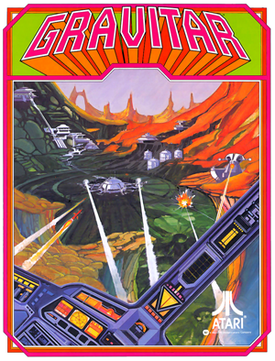
\includegraphics[width=0.32\textwidth]{Gravitar.png}
			\end{center}
			\caption{Gravitar logo}
		\end{wrapfigure}
		
		\section{Gameplay}
	
		The game takes place in a fictional solar system. The player controls a spacecraft with the help of five buttons: two to rotate the ship left and right, one to shoot, one to activate the thruster and one for both a tractor beam and a force field. In the side-view levels, the player has to destroy red bunkers that shoot constantly, and can also use the tractor beam to pick up blue fuel tanks. Once all of the bunkers are destroyed, the planet will blow up, and the player will earn a bonus. Once all planets are destroyed, the player will move onto another solar system.
		The player will lose a life if he crashes into the terrain or gets hit by an enemy's shot, and the game will end immediately if fuel runs out \cite{noauthor_gravitar_2021}.
		
		
		After completing all 11 planets (or alternatively completing the reactor three times) the player enters the second universe and the gravity will reverse. Instead of dragging the ship towards the planet surface, the gravity pushes it away. In the third universe the landscape becomes invisible and the gravity is positive again. The final, fourth universe, has invisible landscape and reverse gravity. After completing the fourth universe the game starts over
		 \cite{noauthor_gravitar_2021}.
		 
		 \pagebreak
		 
		\begin{figure}[ht!]
			\begin{minipage}[c]{0.5\linewidth}
				\centering
				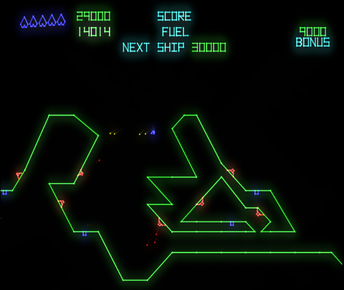
\includegraphics[height=0.3\textheight, width=0.9\linewidth]{Gravitar2.png}
				\caption{A level from Gravitar}
			\end{minipage}\hfill
			\begin{minipage}[c]{0.5\linewidth}	
				\centering
				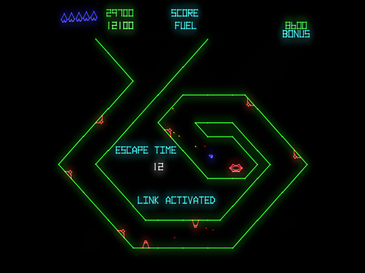
\includegraphics[height=0.3\textheight, width=0.9\linewidth]{Reactor.png}
				\caption{The reactor}
			\end{minipage}
		\end{figure}
	
		\section{Gravitar in SLM-lab}
		
		\emph{SLM-lab} \cite{kenggraesser2017slmlab} is a software framework for reproducible reinforcement learning (RL) research. It implements most of the canonical RL algorithms in a modular platform that allows for easy experimentation and analysis. It includes the OpenAI Gym \cite{brockman2016openai} environments, which contains a lot of Atari games emulations, one being Gravitar.
		
		In this environment, the observation is an RGB image of the screen, which is an array of shape \lstinline|(210, 160, 3)|. Each action is repeatedly performed for a duration of $k$ frames, where $k$ is uniformly sampled from $\{2, 3, 4\}$. The action space is discrete and has 18 available commands like fire, up, down, right, left and so on.
		
		The Gravitar environment can be loaded in SLM-lab by specifying in the \lstinline|.json| configuration file, at the \lstinline|"env"| section the \lstinline|"name"| of the environment. In this case, \lstinline|"GravitarNoFrameskip-v4"|. 
		
	\chapter{Algorithms}
		In this chapter, the algorithms used will be briefly explained.
		\section{Reinforce}
		Reinforce is a Monte Carlo variant of the policy-gradient algorithm in reinforcement learning. The agent collects samples of an episode using its current policy and uses it to update the policy parameter $\theta$. It is updated as an off-policy algorithm:
		\begin{equation}
			\nabla_\theta J(\theta) = E_\pi[G_t \nabla_\theta ln \pi_\theta(a_t, s_t)]
		\end{equation}  
		\section{A2C - Advantage Actor-Critic}
		The Advantage Actor-Critic algorithm relies on two important concepts:
			\paragraph{The Actor-Critic architecture.} This type of algorithms learn two parametrized functions simultaneously. The actor learns the actual policy that the agent uses to act in the world, while the critic learns the value function that evaluates the state-action pairs.
			
			Using the critic to provide a reinforcement signal has the advantage of being able to feed a more continuous signal for training that is useful for example in sparse rewards environments. However, training becomes more difficult because the policy is dependent on the quality of the value function. In the beginning of the training process, the value function is not learned, so the evaluation signal provided doesn't help much to select better actions. Therefore, usually an Advantage function is actually learned.
			\paragraph{Reinforcing signal based on the Advantage function.}
			The advantage function measures how much an action is better or worse than a policy's average action in a certain state. It is defined as follows:
			\begin{equation}
			A^\pi(s_t, a_t) = Q^\pi(s_t, a_t) - V^\pi(s_t)
			\end{equation}
			It has the following properties:
			\begin{itemize}
				\item The advantage is a relative measure. It quantifies whether a particular action $a$ in a state $s$ will improve the policy relative to the value $V^\pi(s)$.
				\item If an action is worse than the average action, but the expected return is still positive - the action taken should become less probable. This is the behavior of the advantage function, in contrast with other methods that might actually encourage that action.
				\item The advantage function is able to capture long-term effects of an action, because it considers all future time steps, while ignoring the effects of all the actions to date. 
			\end{itemize}
			\subsection{Estimating the advantage with n-Step returns}
			The n-Step estimate is formulated as follows:
			\begin{equation}
				A_{Nstep}^\pi (s_t, a_t) = Q^\pi(s_t, a_t) - V^\pi(s_t) \approx r_t + \gamma r_{t+1} + \gamma^2 r_{t+2} + \dots + \gamma^n r_{t + n} + \gamma^{n_+ 1} \hat{V}^\pi(s_{t+n + 1}) - \hat{V}^\pi(s_t)
			\end{equation}
			The hyperparameter n - the number of actual rewards, controls the bias-variance trade-off.
			\subsection{Estimating the advantage with Generalized Advantage Estimation}
			GAE is defined as an exponentially weighted average of all of the n-step forward return advantages:
			\begin{equation}
				A_{GAE}^\pi (s_t, a_t) = \sum_{l=0}^{\infty}(\gamma \lambda)^l \delta_{t+l}
			\end{equation}
			where, $\delta_t = r_t + \gamma V^\pi (s_{t+1}) - V^\pi (s_t)$
			
			The variance is controlled through the decay coefficient $\lambda$
		\section{PPO - Proximal Policy Optimization}
		PPO \cite{schulman_proximal_2017} aims at avoiding the problem of performance collapse through a surrogate objective that is guaranteed to have monotonic improvement. 
		It works by extending either REINFORCE or an actor-critic algorithm with the modified objective. It is data efficient and reliable as TRPO \cite{schulman_trust_2017} but uses first-order optimization.
		Let $r_t(\theta)$ denote the probability ratio $r_t(\theta) = \frac{\pi_\theta(a_t|s_t)}{\pi_{\theta_{old}}(a_t|s_t)}$ so r($\theta_{old}) = 1$. TRPO maximizes a "surrogate" objective: 
		\begin{equation}
			L^{CPI}(\theta) = \hat{E}_t \left[\frac{\pi_\theta(a_t | s_t)}{\pi_{\theta_{old}}(a_t | s_t)}\hat{A}_t\right] = \hat{E}_t\left[r_t(\theta)\hat{A}_t\right]
		\end{equation}
		where $CPI$ refers to a conservative policy iteration.\cite{schulman_proximal_2017}
		Without a constraint, maximization of $L^{CPI}$ would lead to an excessively large policy update, therefore, PPO modifies the objective to penalize changes to the policy that moves $r_t(\theta)$ away from 1:
		\begin{equation}
			J^{CLIP}(\theta) = \hat{E}\left[ min \left( r_t(\theta)\hat{A}, clip\left( r_t(\theta), 1 - \epsilon, 1 + \epsilon \right) \hat{A} \right) \right]
		\end{equation}
		where $\epsilon$ is a hyperparameter. The intuition is as follows: The $clip$ term modifies the surrogate objective by clipping the probability ratio, which removes the incentive to move $r_t$ outside the interval $[1-\epsilon, 1 + \epsilon]$ \cite{schulman_proximal_2017}.
		
		
	\chapter{Experimental Results}
	\section{Reinforce}
	
	For training Reinforce, the following configuration has been used:
	\begin{lstlisting}
		{
			"reinforce_gravitar": {
				"agent": [{
					"name": "Reinforce",
					"algorithm": {
						"name": "Reinforce",
						"action_pdtype": "default",
						"action_policy": "default",
						"center_return": true,
						"explore_var_spec": null,
						"gamma": 0.99,
						"entropy_coef_spec": {
							"name": "linear_decay",
							"start_val": 0.01,
							"end_val": 0.001,
							"start_step": 1000,
							"end_step": 300000
						},
						"training_frequency": 1
					},
					"memory": {
						"name": "OnPolicyReplay",
						"batch_size": 64
					},
					"net": {
						"type": "ConvNet",
						"shared": true,
						"conv_hid_layers": [
						[32, 8, 4, 0, 1],
						[64, 4, 2, 0, 1],
						[32, 3, 1, 0, 1]
						],
						"fc_hid_layers": [512],
						"hid_layers_activation": "relu",
						"init_fn": "orthogonal_",
						"normalize": true,
						"batch_norm": false,
						"clip_grad_val": 0.5,
						"loss_spec": {
							"name": "MSELoss"
						},
						"optim_spec": {
							"name": "Adam",
							"lr": 0.002
						},
						"lr_scheduler_spec": null,
						"gpu": true
					}
				}],
				"env": [{
					"name": "GravitarNoFrameskip-v4",
					"frame_op": "concat",
					"frame_op_len": 4,
					"reward_scale": "sign",
					"num_envs": 16,
					"max_t": null,
					"max_frame": 300000
				}],
				"body": {
					"product": "outer",
					"num": 1
				},
				"meta": {
					"distributed": false,
					"eval_frequency": 10000,
					"max_session": 1,
					"max_trial": 1
				}
			}
		}
	\end{lstlisting}

	The following parameters are set:
		\begin{itemize}
	\item The algorithm is set to Reinforce
	\item The action policy is the default one
	\item The agent uses a convolutional network with three layers connected to a single linear layer with ReLU activations.
	\item The optimizer is Adam.
	\item Algorithm is trained for 300k steps.
	\item Evaluation occurs every 10k steps.
	
	The following returns are obtained:
	
	\begin{figure}[ht!]
		\begin{minipage}[c]{0.5\linewidth}
			\centering
			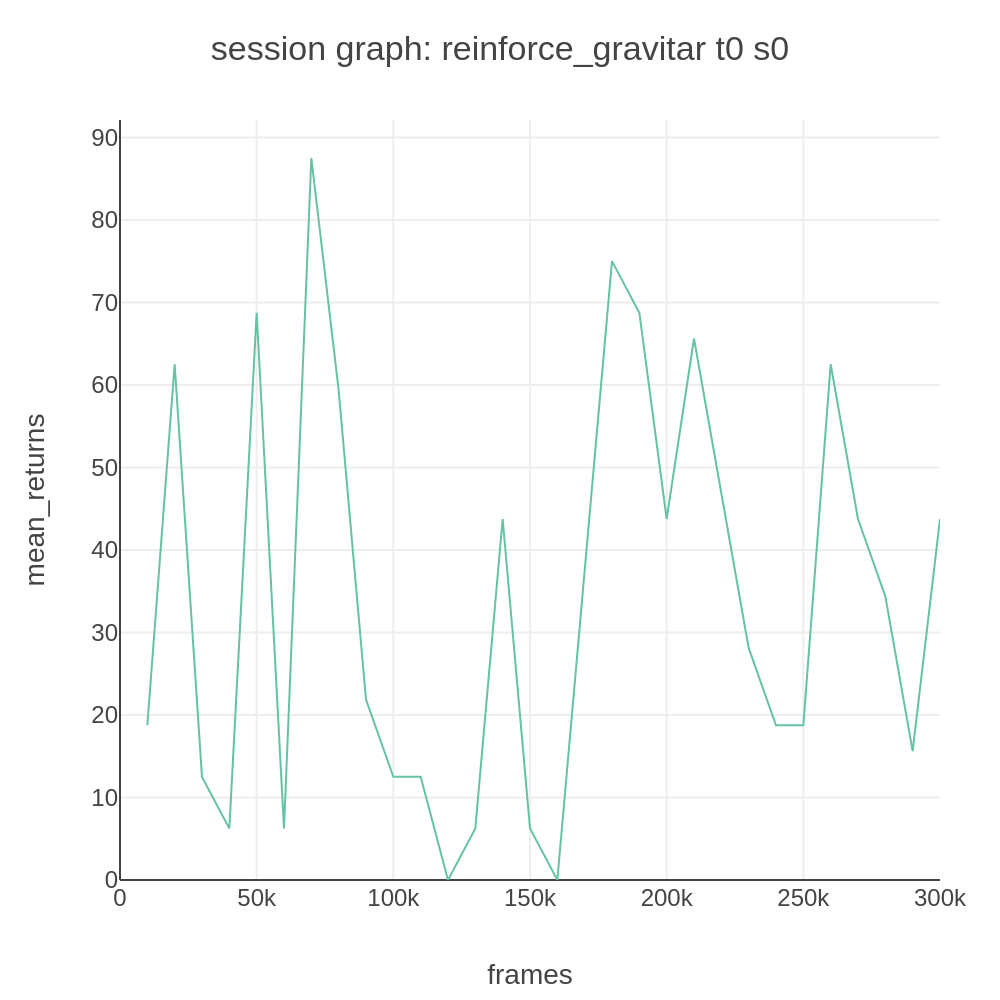
\includegraphics[height=0.3\textheight, width=0.9\linewidth]{reinforce_gravitar_t0_s0_session_graph_eval_mean_returns_vs_frames.png}
			\caption{Trial graph}
		\end{minipage}\hfill
		\begin{minipage}[c]{0.5\linewidth}	
			\centering
			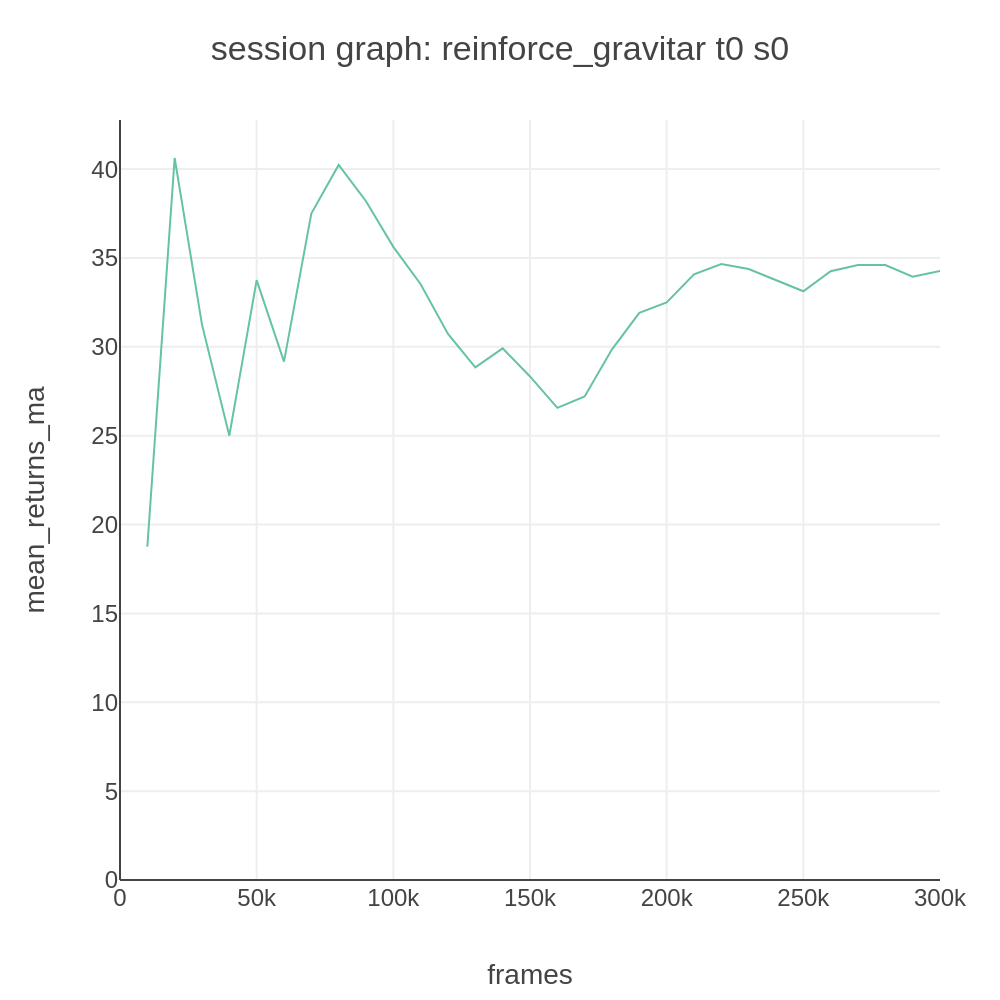
\includegraphics[height=0.3\textheight, width=0.9\linewidth]{reinforce_gravitar_t0_s0_session_graph_eval_mean_returns_ma_vs_frames.png}
			\caption{Trial graph with moving average}
		\end{minipage}
		\caption{Reinforce trial graphs from SLM lab. On the vertical axis the total rewards are shown and on the horizontal axis the number of frames.}
	\end{figure}
	
\end{itemize}
	
	\section{A2C}
	
	For training A2C, two experiments have been considered: 
	\begin{enumerate}
		\item Training with generalized advantage function (GAE)
		The config file is as follows:
		
		\begin{lstlisting}
			{
				"a2c_gae_gravitar": {
					"agent": [{
						"name": "A2C",
						"algorithm": {
							"name": "ActorCritic",
							"action_pdtype": "default",
							"action_policy": "default",
							"explore_var_spec": null,
							"gamma": 0.99,
							"lam": 0.95,
							"num_step_returns": null,
							"entropy_coef_spec": {
								"name": "no_decay",
								"start_val": 0.01,
								"end_val": 0.01,
								"start_step": 0,
								"end_step": 0
							},
							"val_loss_coef": 0.5,
							"training_frequency": 32
						},
						"memory": {
							"name": "OnPolicyBatchReplay"
						},
						"net": {
							"type": "ConvNet",
							"shared": true,
							"conv_hid_layers": [
							[32, 8, 4, 0, 1],
							[64, 4, 2, 0, 1],
							[32, 3, 1, 0, 1]
							],
							"fc_hid_layers": [512],
							"hid_layers_activation": "relu",
							"init_fn": "orthogonal_",
							"normalize": true,
							"batch_norm": false,
							"clip_grad_val": 0.5,
							"use_same_optim": false,
							"loss_spec": {
								"name": "MSELoss"
							},
							"actor_optim_spec": {
								"name": "RMSprop",
								"lr": 7e-4,
								"alpha": 0.99,
								"eps": 1e-5
							},x
							"critic_optim_spec": {
								"name": "RMSprop",
								"lr": 7e-4,
								"alpha": 0.99,
								"eps": 1e-5
							},
							"lr_scheduler_spec": null,
							"gpu": true
						}
					}],
					"env": [{
						"name": "GravitarNoFrameskip-v4",
						"frame_op": "concat",
						"frame_op_len": 4,
						"reward_scale": "sign",
						"num_envs": 16,
						"max_t": null,
						"max_frame": 1e6
					}],
					"body": {
						"product": "outer",
						"num": 1
					},
					"meta": {
						"distributed": false,
						"eval_frequency": 10000,
						"log_frequency": 10000,
						"rigorous_eval": 0,
						"max_session": 1,
						"max_trial": 1
					}
				}
			}
		\end{lstlisting}
	
		The following parameters are set:
		\begin{itemize}
			\item The algorithm is A2C
			\item The action policy is the default one
			\item GAE is used as an Advantage function estimator
			\item The agent uses a convolutional network with three layers connected to a single linear layer with ReLU activations.
			\item The optimizer is RMSProp.
			\item Algorithm is trained for 1M steps.
			\item Evaluation occurs every 10k steps.
		\end{itemize}
	
		The following returns are obtained:
		
		\begin{figure}[ht!]
			\begin{minipage}[c]{0.5\linewidth}
				\centering
				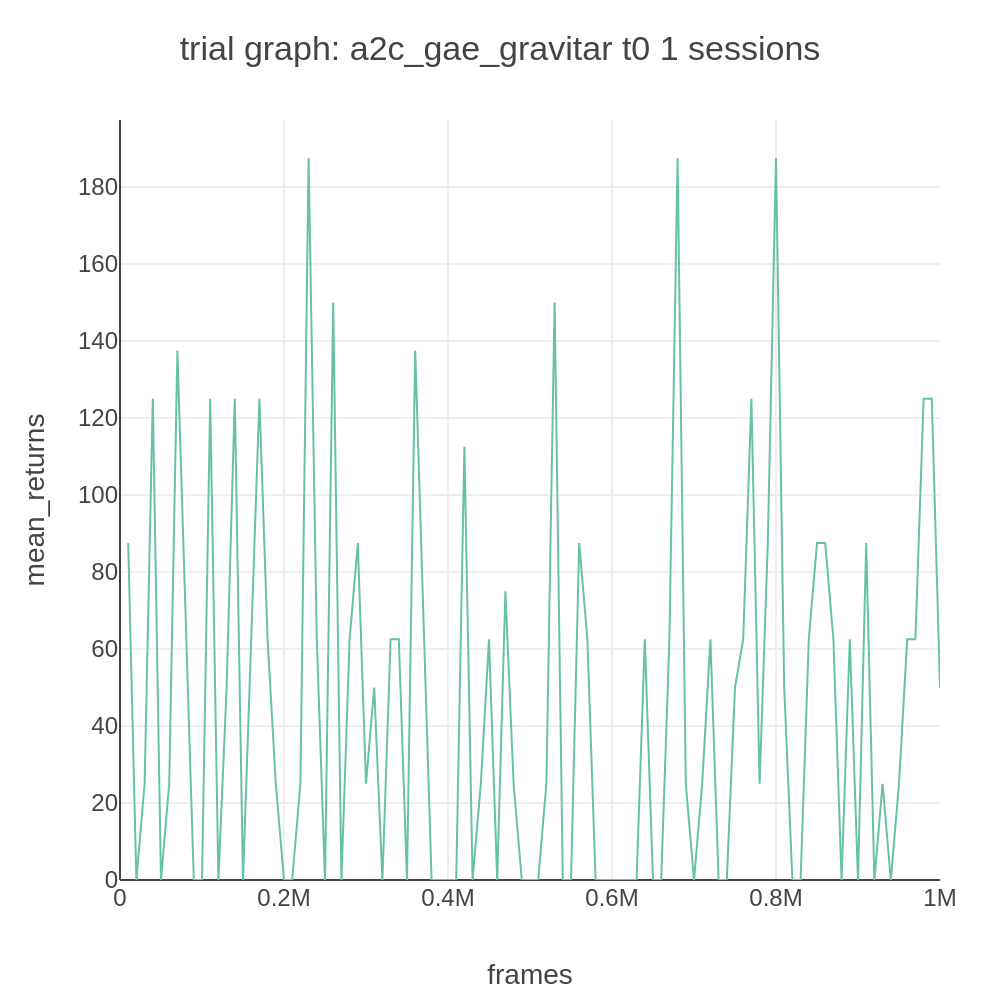
\includegraphics[height=0.3\textheight, width=0.9\linewidth]{a2c_gae_gravitar_t0_trial_graph_mean_returns_vs_frames.png}
				\caption{Trial graph}
			\end{minipage}\hfill
			\begin{minipage}[c]{0.5\linewidth}	
				\centering
				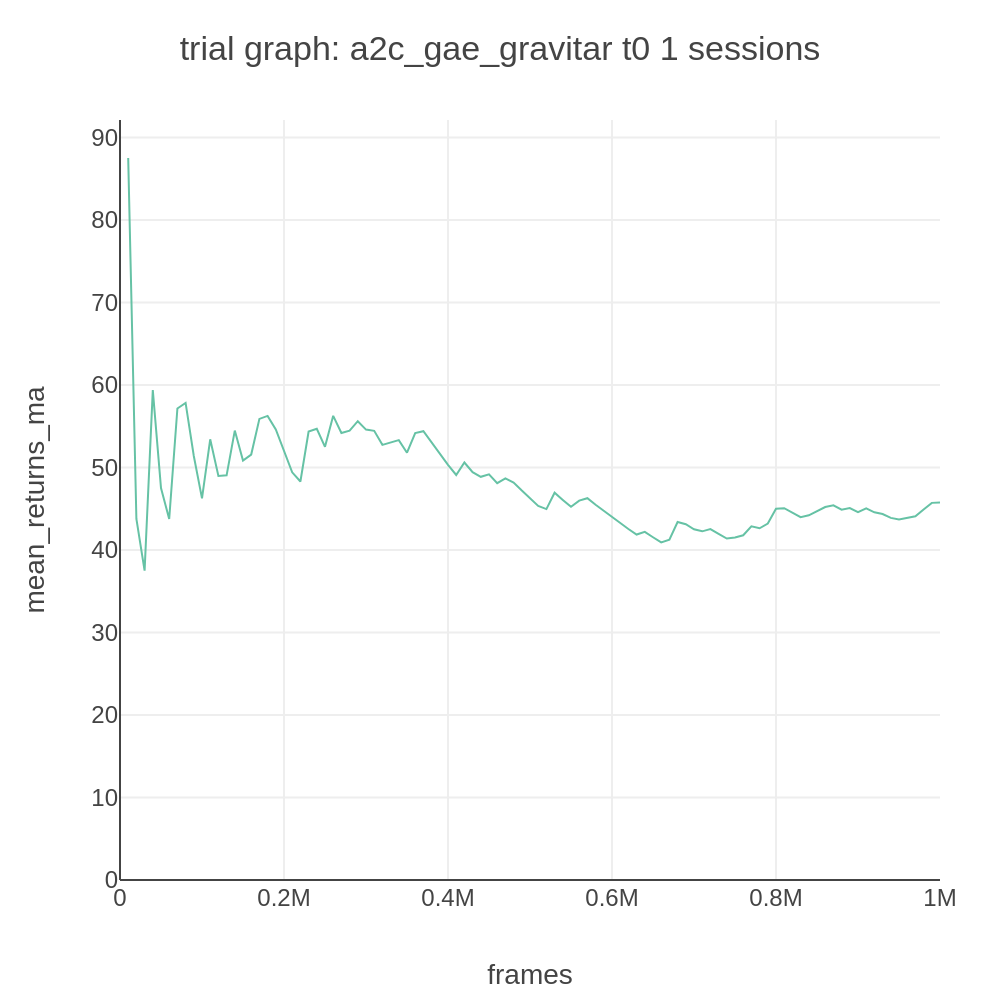
\includegraphics[height=0.3\textheight, width=0.9\linewidth]{a2c_gae_gravitar_t0_trial_graph_mean_returns_ma_vs_frames.png}
				\caption{Trial graph with moving average}
			\end{minipage}
			\caption{A2C trial graphs from SLM lab. On the vertical axis the total rewards are shown and on the horizontal axis the number of frames.}
			\end{figure}
		
		\pagebreak
		\item Training with n-Step Returns
		
		The config file is almost the same as the GAE version, it differs at the $num\_step\_returns$ parameter.
		
		The following returns are obtained:
		
		\begin{figure}[ht!]
			\begin{minipage}[c]{0.5\linewidth}
				\centering
				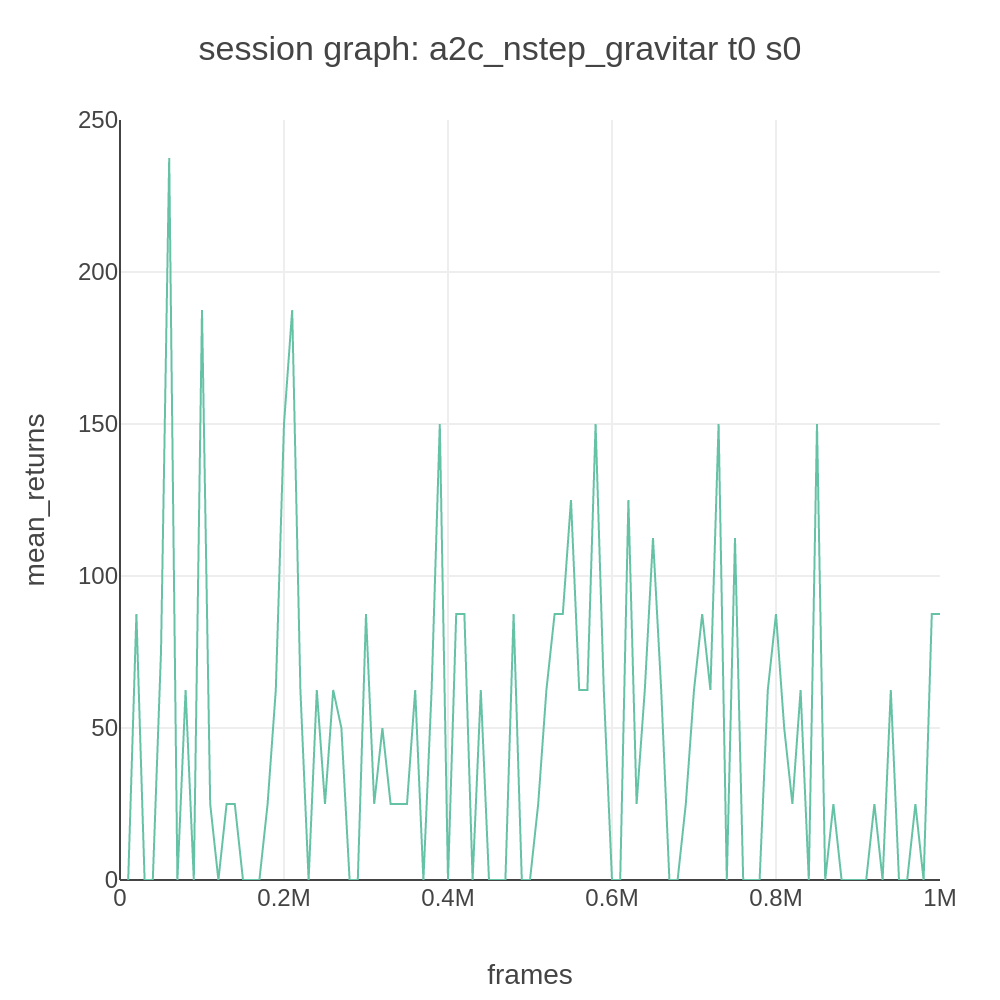
\includegraphics[height=0.3\textheight, width=0.9\linewidth]{a2c_nstep_gravitar_t0_s0_session_graph_eval_mean_returns_vs_frames.png}
				\caption{Trial graph}
			\end{minipage}\hfill
			\begin{minipage}[c]{0.5\linewidth}	
				\centering
				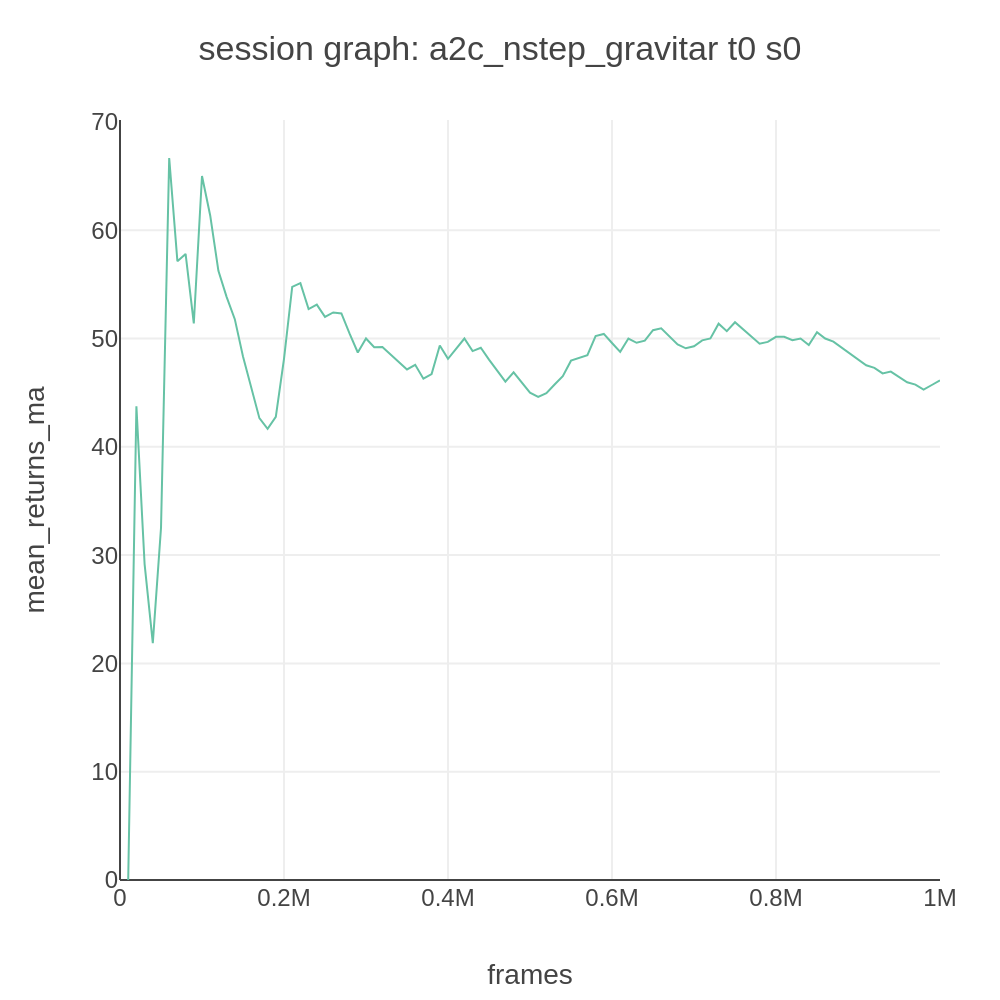
\includegraphics[height=0.3\textheight, width=0.9\linewidth]{a2c_nstep_gravitar_t0_s0_session_graph_eval_mean_returns_ma_vs_frames.png}
				\caption{Trial graph with moving average}
			\end{minipage}
			\caption{A2C trial graphs from SLM lab. On the vertical axis the total rewards are shown and on the horizontal axis the number of frames.}
		\end{figure}
	\end{enumerate}
	
	\section{PPO}
	
	For training the Proximal Policy Optimization algorithm, the following configuration has been used:
	\begin{lstlisting}
		{
			"ppo_gravitar": {
				"agent": [{
					"name": "PPO",
					"algorithm": {
						"name": "PPO",
						"action_pdtype": "default",
						"action_policy": "default",
						"explore_var_spec": null,
						"gamma": 0.99,
						"lam": 0.70,
						"clip_eps_spec": {
							"name": "no_decay",
							"start_val": 0.10,
							"end_val": 0.10,
							"start_step": 0,
							"end_step": 0
						},
						"entropy_coef_spec": {
							"name": "no_decay",
							"start_val": 0.01,
							"end_val": 0.01,
							"start_step": 0,
							"end_step": 0
						},
						"val_loss_coef": 0.5,
						"time_horizon": 128,
						"minibatch_size": 256,
						"training_epoch": 4
					},
					"memory": {
						"name": "OnPolicyBatchReplay",
					},
					"net": {
						"type": "ConvNet",
						"shared": true,
						"conv_hid_layers": [
						[32, 8, 4, 0, 1],
						[64, 4, 2, 0, 1],
						[32, 3, 1, 0, 1]
						],
						"fc_hid_layers": [512],
						"hid_layers_activation": "relu",
						"init_fn": "orthogonal_",
						"normalize": true,
						"batch_norm": false,
						"clip_grad_val": 0.5,
						"use_same_optim": false,
						"loss_spec": {
							"name": "MSELoss"
						},
						"actor_optim_spec": {
							"name": "Adam",
							"lr": 2.5e-4,
						},
						"critic_optim_spec": {
							"name": "Adam",
							"lr": 2.5e-4,
						},
						"lr_scheduler_spec": {
							"name": "LinearToZero",
							"frame": 1e7
						},
						"gpu": true
					}
				}],
				"env": [{
					"name": "GravitarNoFrameskip-v4",
					"frame_op": "concat",
					"frame_op_len": 4,
					"reward_scale": "sign",
					"num_envs": 4,
					"max_t": null,
					"max_frame": 1e6
				}],
				"body": {
					"product": "outer",
					"num": 1
				},
				"meta": {
					"distributed": false,
					"eval_frequency": 10000,
					"log_frequency": 10000,
					"rigorous_eval": 0,
					"max_session": 1,
					"max_trial": 1
				}
			}
		}
	\end{lstlisting}
	
	The following parameters are set:
	\begin{itemize}
		\item The action policy is the default policy for a discrete action space.
		\item Generalized advantage estimation is used.
		\item The clipping parameters are set in lines 12-17
		\item In the lines 34-43 the network architecture is set as a 3 layer convolutional network with a hidden fully connected layer and ReLU activations.
		\item The opimizer is set to Adam both for the actor and the critic networks.
		\item The environment is Gravitar.
		\item Evaluation is done every 10k steps.
		\item The algorithm is trained for 1M steps.
	\end{itemize}
	 \pagebreak
	The following returns are obtained:
	
	\begin{figure}[ht!]
		\begin{minipage}[c]{0.5\linewidth}
			\centering
			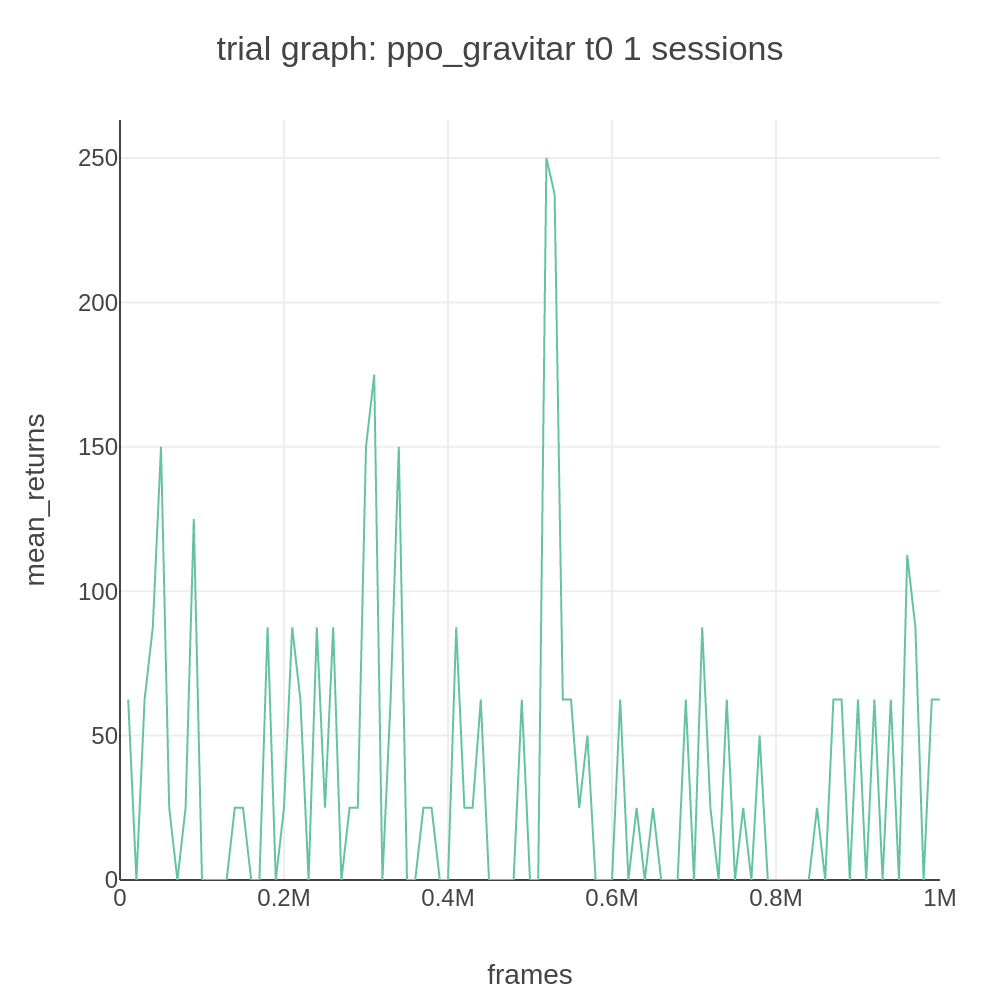
\includegraphics[height=0.3\textheight, width=0.9\linewidth]{ppo_gravitar_t0_trial_graph_mean_returns_vs_frames.png}
			\caption{Trial graph}
		\end{minipage}\hfill
		\begin{minipage}[c]{0.5\linewidth}	
			\centering
			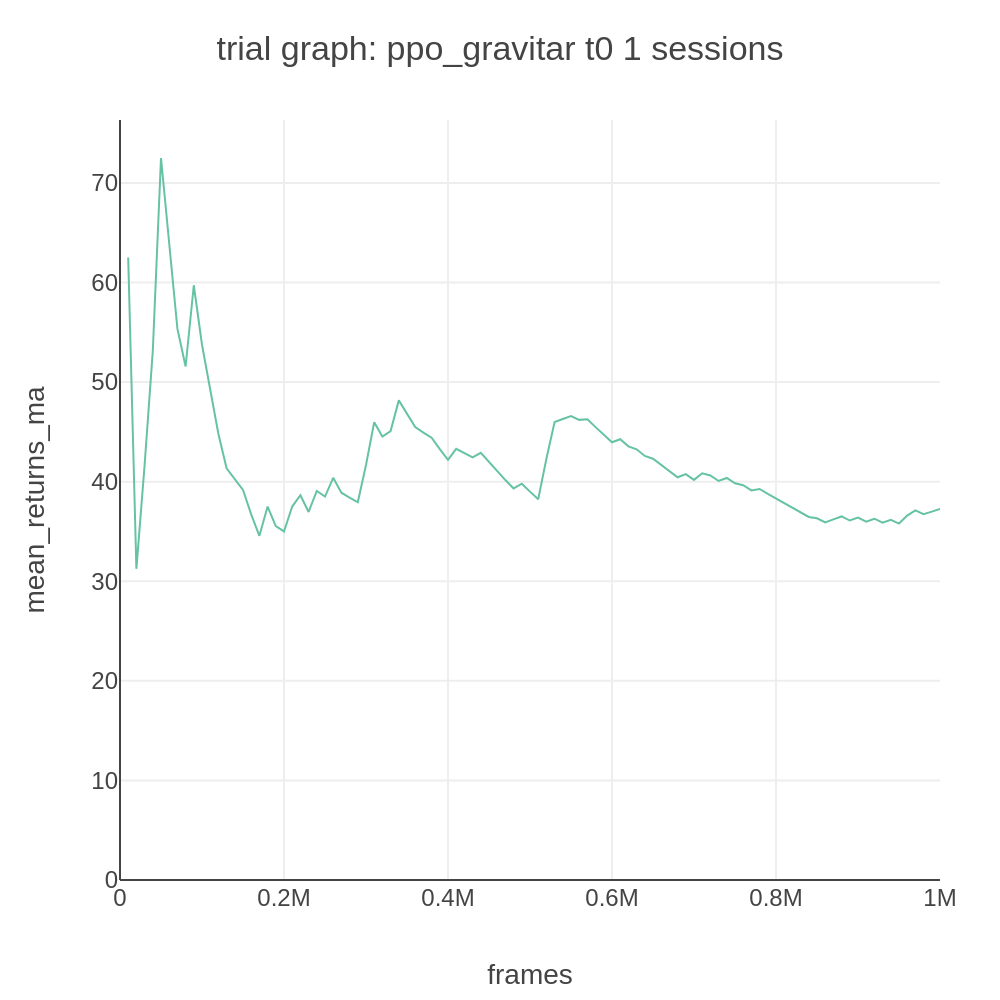
\includegraphics[height=0.3\textheight, width=0.9\linewidth]{ppo_gravitar_t0_trial_graph_mean_returns_ma_vs_frames.png}
			\caption{Trial graph with moving average}
		\end{minipage}
		\caption{PPO trial graphs from SLM lab. On the vertical axis the total rewards are shown and on the horizontal axis the number of frames.}
	\end{figure}
	\chapter{Conclusions}
	
	To conclude, Gravitar is a very difficult game to solve. Not only due to it's more complex physics and controls, but also due to the fact that the levels are increasingly difficult and quite different from one to another. No algorithms from the ones tested was able to decently solve this environment. As a comparison, apart from Reinforce, which (with no surprise) performed the poorest, the other algorithms performed similarly, with the n-step A2C having the best mean returns average of approx. 50. Also, all the algorithms suffered performance degradation as more steps were taken. 
	
	\bibliographystyle{unsrt}	% Order by citation
	\bibliography{lab_report_bibliography.bib}
	
\end{document}